\section{Résolution numérique}

Dans cette partie, nous allons expliquer comment le problème se résout
numériquement et aborder quelques considérations en rapport avec cette
résolution.

\subsection{Principe de la résolution}
La résolution peut être découpée en plusieurs partie, plus ou moins
indépendantes.

Une première considération numérique est la discrétisation spatiale du problème
: le disque sera représenté par un ensemble de position discrète selon l’axe
radial. Ces positions s’étendent de $x_\textrm{min} = \sqrt{r_\textrm{min}/r_s}$ à $x_\textrm{max} =
\sqrt{r_\textrm{max}/r_s}$, et sont séparées par un $\mathrm{d} x$ constant, ce qui aura pour
effet une fois revenu dans le monde dimensionné d’avoir un $\mathrm{d} r$ parabolique,
avec donc plus de points vers le bord intérieur du disque et moins vers le bord
extérieur. Comme l'instabilité commence par se développer au niveau du bord intérieur, il est favorable d'y avoir un bon échantillonnage.

La simulation commence dans le régime en évolution stable et avec des
paramètres tels qu'un régime stationnaire existe. Le disque va alors rapidement
se stabiliser thermiquement jusqu'à atteindre la courbe en S avant de converger
sur un temps visqueux vers l'état stationnaire. Une fois l'état stationnaire
atteint, le flux de matière est augmenté. On recommence alors à suivre la
courbe en S jusqu'à atteindre un nouveau régime stationnaire.

Lorsque le flux de matière entrant est trop élevé, il n'existe plus de régime
stationnaire mais seulement un régime en évolution instable. Les points proches
des points critiques commencent alors à effectuer des cycles d'amplitude
croissante jusqu'à déclencher l'instabilité. Une fois l'instabilité terminée,
la densité et la température sont de nouveau assez faible pour retomber dans un
régime d'évolution stable.

\subsubsection{Courbe en S}

L’idée ici est de trouver les zones de stationnarité du système, c’est-à-dire
celles pour lesquelles la température évolue peu. Cela revient à résoudre
l’équation $Q^+ = Q^-$. En pratique, cette courbe a une forme « en S », avec
une partie arrondie correspondant au cas optiquement épais et une partie droite
correspondant au cas optiquement mince. Il y a deux points critiques : un au
point extrême de la partie arrondie, appelé premier point critique, et un au
point de jonction des deux parties, appelé second point critique.

Il faut donc déterminer la courbe de stationnarité en chaque point du disque,
puis sortir les coordonnées des points critiques pour chacun d’entre eux ainsi
que déterminer une position initiale pour le système sur ces courbes. Le détail de 
cette résolution sont donnés dans la partie \ref{sec:courbe_s}.

\subsubsection{Domaines de la simulation}

Le disque à un moment $t$ peut être dans l'une des trois situations suivantes.

\paragraph{Régime stationnaire} ce régime correspond au disque dans une
situation telle que tout le flux de matière entrant traverse le disque pour
finir par tomber dans le trou noir. Il est caractérisé par une température et
une densité surfacique constantes au cours du temps. Le taux d'accrétion est
alors constant et égal au taux d'accrétion à son bord extérieur. Numériquement,
il se traduit par une évolution relative de $T$ et $S^\star$ très faible entre
deux pas de temps. 

\paragraph{Régime en évolution stable} ce régime correspond au disque évoluant
sur un temps visqueux pour la densité surfacique et un temps thermique pour la
température. Dans ce régime, on pourra négliger le terme advectif du chauffage.
Ce régime se situe dans la partie inférieure de la courbe en S et est
caractérisé par un quasi-équilibre thermique. On aura donc $Q^+ = Q^-$. Dans un
diagramme $\Sigma-T$ (figure \ref{fig:qmap}), ce régime correspond au suivi de la partie inférieure
droite de la courbe en S. 

\paragraph{Régime en évolution instable} ce régime est celui de l'instabilité.
Il est caractérisé par une évolution de la densité surfacique et de la
température sur un même temps thermique. Dans ce régime, au moins une partie du
disque se situe à une température ou une densité de surface plus élevée que les
valeurs critiques. L'équilibre thermique n'y est alors pas atteint. C'est là
que se situe le cœur du problème. Le disque évacue de l'énergie par rayonnement
et perd beaucoup de matière par chute dans le trou noir. Chaque point proche du
point critique va effectuer des cycles autour du point critique. Ces points
voient d'abord leur densité augmentée jusqu'à dépasser la densité critique. Au
dela, la température croît rapidement jusqu'à ce que l'advection ne soit plus
négligeable et limite la température tout en diminuant la densité localement.
Le point se dirige alors vers les densités faibles, au dessus du point critique
jusqu'à retraverser la courbe en S, où le refroidissement est plus important
que le chauffage. Le point retombe alors dans la partie inférieure de la courbe
en S. \\

\begin{figure}[!ht]
    \centering
    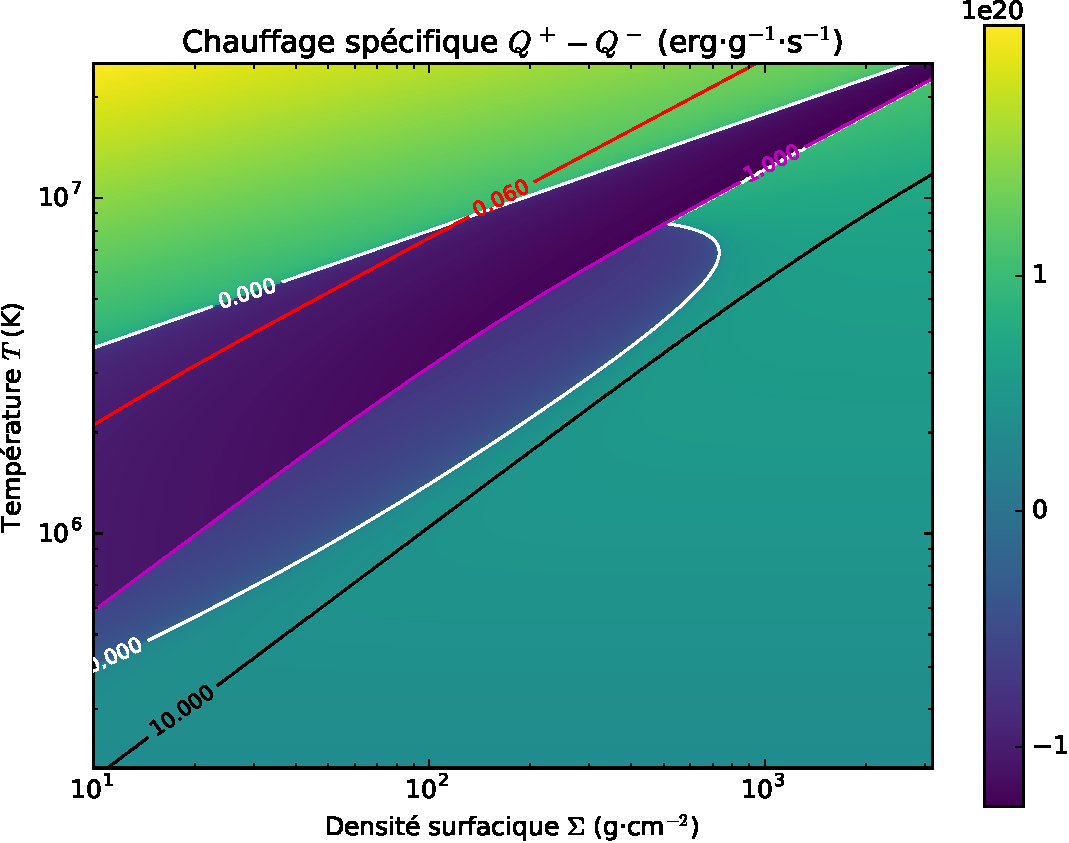
\includegraphics[width=\textwidth]{Qmap.pdf}
    \caption{Carte de la différence des termes de chauffages et de refroidissement en fonction de $T$ et $\Sigma$}
    \label{fig:qmap}
\end{figure}

Sur la \cref{fig:qmap} on aperçoit bien les différentes zones du problèmes et
le comportement du système se prédit bien. On observe d’ailleurs que la courbe
en S est fortement modifiée par la prise en compte effective de l’opacité : la
partie basse se voit bien, la partie haute (droite blanche supérieure)
également, mais la jonction entre les deux ne se fait pas.

En commençant dans la partie correspondant au régime en évolution stable, tout point est amené à se
retrouver sur la partie basse de la courbe en S, puisqu’il est chauffé si
en-dessous et refroidi si au-dessus. Ensuite, avec l’accrétion de matière, le
système va remonter le long de cette courbe jusqu’à arriver au premier point
critique. Si lors de cette ascention le système se place dans un régime stationnaire, nous augmentons le flux de
matière entrant au bord externe et ce jusqu'à ce qu'il repasse au régime en évolution stable.

Au moment ou le point critique est atteint, plus rien ne l’empêche de monter en température, ce
qu’il va donc faire. Dans cette zone, la convection n’est plus négligeable, car
les points du système ne sont plus tous concentrés dans la même zone
d’évolution. On est donc au régime en évolution instable, qui va se traduire par la propagation d'une instabilité sous la forme d’un pic
de densité de matière et d’un front de température : la matière en trop au
centre va partir vers l’extérieur, poussant les points restés en bas à droite
du point critique ; ils iront donc rejoindre les autres sur la branche haute.

Cette évolution s’arrête en effet pour tout point dès lors qu’il atteint la
frontière $\tau_{eff} = 1$. Au-dessus de cette barrière le terme de
refroidissement reprend le dessus fortement, et les points se figent.

Puis, une fois l’instabilité dissipée, le système va se refroidir
progressivement en redescendant le long de la droite $\tau_{eff} = 1$, jusqu’à
retomber à « l’intérieur » de la courbe en S. À ce moment-là, plus rien
n’empêche les points de redescendre en température, et ils vont donc retomber
sur la partie basse de la courbe correspondant au régime en évolution stable.


\subsubsection{Considérations sur les dérivées numériques spatiales}

Dans un certain nombre d’équations interviennent plusieurs dérivées spatiales,
du premier ou second ordre. Il existe plusieurs manières de les calculer
numériquement, ayant des conséquences variées. Nous nous intéresserons à
celles-ci dans cette partie afin d’expliquer les choix effectués.

\subsubsection{Conditions aux bords}

Toujours à propos des dérivées spatiales intervenant, l’existence de bords «
numériques » au problème implique d’imposer des conditions aux bords pour ces
dernières. Ces conditions dépendent des dérivées numériques utilisées, dans
cette partie seront présentées uniquement celles intervenant pour les dérivées
effectivement utilisées, les autres seront présentées en ANNEXE CL.
%TODO: Annexe CL

\subsubsection{Intégration numérique de $S^\star$ et $T^\star$}

L'évolution du disque d'accrétion est dominé par les deux équations sur
$S^\star$ \eqref{eq:difS} et sur $T^\star$ \eqref{eq:difT}.

Les régimes stationnaires et en évolution stable seront traités avec un schéma
explicite pour la température et un schéma implicite pour la densité de
surface. On a alors un temps visqueux $\tau_\nu$ (voir section \ref{sec::pas_de_temps}) très grand devant le temps
thermique $\tau_T$. On peut donc intégrer $S^\star$ et $T$ sur deux échelles de
temps différentes et effectuer une démarche de ``step and relax'', où on
intègre d'abord $S^\star$ sur un grand temps (visqueux) avant de laisser se
relaxer $T$ sur des petits temps (thermiques). Il faut à cet endroit faire
attention à ce que le temps de relaxation de $T$ soit toujours plus petit que
le temps visqueux. Cela revient à vérifier que le nombre d'itérations
nécessaires à la stabilisation de $T$ est plus petit que
$\nicefrac{\tau_\nu}{\tau_T}$. Si cette condition est violée, la simulation
numérique ne traduit plus de réalité physique. 

Une méthode implicite pour $S^\star$ est alors préconisée. En effet, celle-ci
assure de converger vers la solution et est stable quelque soit le pas de temps
(dans la limite des approximations données précédemment). Les détails de la
méthode sont donnés dans la partie \ref{ssec:integration_S_imp}. Pour intégrer
la température, il n'est pas possible d'écrire un schéma implicite. Il faudra
donc utiliser un schéma explicite. En revanche, il sera possible de procéder à
des simplifications pour donner une convergence plus rapide de $T$. Les détails
de ces approximations sont donnés dans la partie \ref{ssec:integration_T}.

L'autre régime est instable. Les évolutions de $S^\star$ et de $T$ se font sur
des temps similaires. Dans ce régime, il n'est plus légitime de traiter
séparement ces deux variables et il faut donc résoudre conjointement l'une et
l'autre. Le schéma implicite n'y est pas utilisé, car il n'assure que la
convergence vers une solution physique, mais pas via des états successifs
physiquement acceptables. Comme la valeur de $S^\star$ influe sur celle de $T$,
cela impliquerait que l'intégration de $T$ n'est pas non plus exacte. Dans le
cas du comportement chaotique de l'instabilité, il est nécessaire de limiter au
maximum les erreurs numériques car celles-ci peuvent mener à un résultat final
différent du résultat physiquement attendu. Le choix d'un schéma explicite est
alors fait pour $T$ et $S^\star$, les deux évoluant alors sur le plus petit
temps charactéristique du système : le pas de temps thermique. Le schéma
explicite est donné dans la partie \ref{ssec:integration_S_exp} pour $S^\star$
et dans la partie \ref{ssec:integration_T} pour $T$.

\subsubsection{Détermination du pas de temps\label{sec::pas_de_temps}}

Nous allons expliciter dans cette section les choix que nous avons fait pour
déterminer les différents pas de thermique $\tau_T$ et visqueux $\tau_\nu$
nécessaires aux intégrations en schéma implicite et explicite.

Sur la première branche (intégration en schéma implicite), ils sont déterminés
au cours de la simulation avant chaque nouvelle intégration en $S^\star$, à
partir des formules suivantes : 

\begin{equation}
	\Delta \tau_\nu^{imp} = \frac{\tau_\nu}{k_{\nu}} = \frac{1}{k_{\nu}} \times \frac{r}{v}
\end{equation}

\begin{equation}
	\Delta \tau_{T}^{imp} = \frac{\tau_{T}}{k_{T}}= \frac{1}{k_{T}} \times \frac{C_{V} T}{Q^{+} - Q^{-}}
\end{equation} \\

où $k_{\nu}$ et $k_{T}$ sont des constantes que l'on à prise respectivement égales à 100 et 1000.

Il est nécessaire dans cette simulation de faire intervenir un pas de temps
adaptatif. En effet, l'approche du point critique que l'on peut voir en figure
\ref{Fig::bench} est délicate. Le pas de temps visqueux est donc multiplier à
chaque nouvelle intégration sur $S^\star$ par un facteur $\alpha$ dépendant de la
distance au point critique par rapport à la variable $S^\star$. L'évolution du facteur $\alpha$ en fonction de la densité de surface $\Sigma$ est représenté figure \ref{fig::alpha_fct_sig} 


\begin{equation}
	\Delta^{'} \tau_{\nu}^{imp} = \alpha \Delta \tau_{\nu}^{imp}
\end{equation} \\

où $\alpha = 1 - \left( 0.99 \times \e^{- \left| \frac{S_\textrm{crit} - S}{D_\textrm{crit}} \right|} \right)$, avec $D_\textrm{crit}$ défini arbitrairement : $D_\textrm{crit} = 200$.


\begin{figure}
  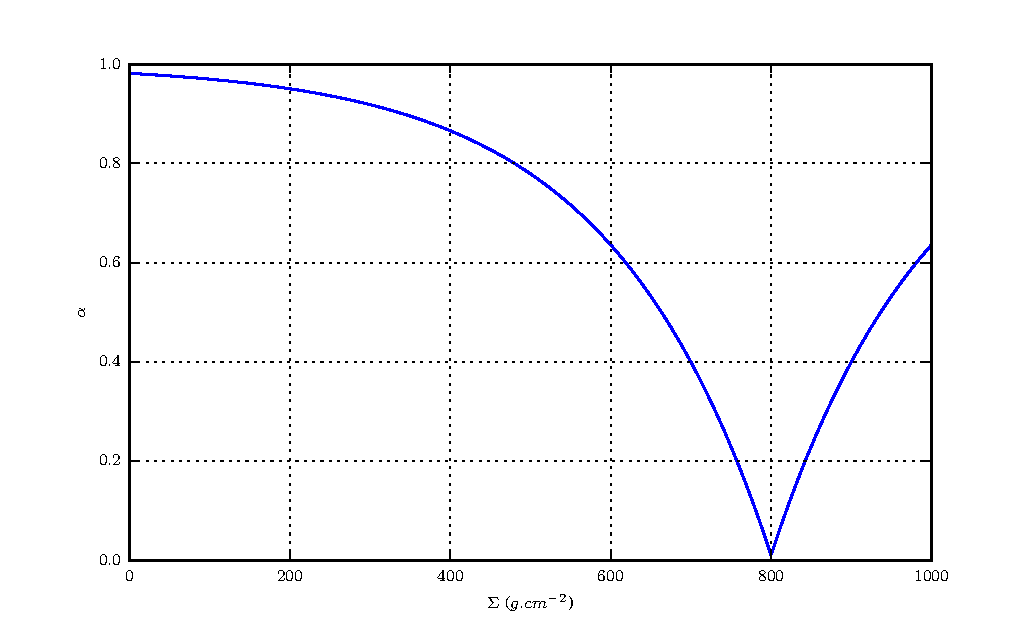
\includegraphics{figures/alpha_fonction_de_sigma.pdf}
  \caption{Evolution du facteur de ralentissement $\alpha$ en fonction de la densité de surface $\Sigma$ - Le point de rupture représente la valeur de $\Sigma$ au point critique}
  \label{fig::alpha_fct_sig}
\end{figure}

Le passage en shéma d'intégration explicite est soumis à deux conditions : $T
\ge T_\textrm{crit}$ ou $\Sigma \ge \Sigma_\textrm{crit}$. On bascule dès lors
qu'un des rayons à rempli ces conditions. $T$ et $\Sigma$ sont alors intégrés
sur le même pas de temps :

\begin{equation}
\Delta \tau_{T}^{exp} = 0.01 \times \Delta \tau_{T}^{imp}
\end{equation}

\subsubsection{Calcul des autres variables}

